%–––––––––––––––––––––––––––––––––––––––––––––––
% Figure 1: Number of Terrorist Attacks per Year
\begin{figure}[ht]
  \centering
  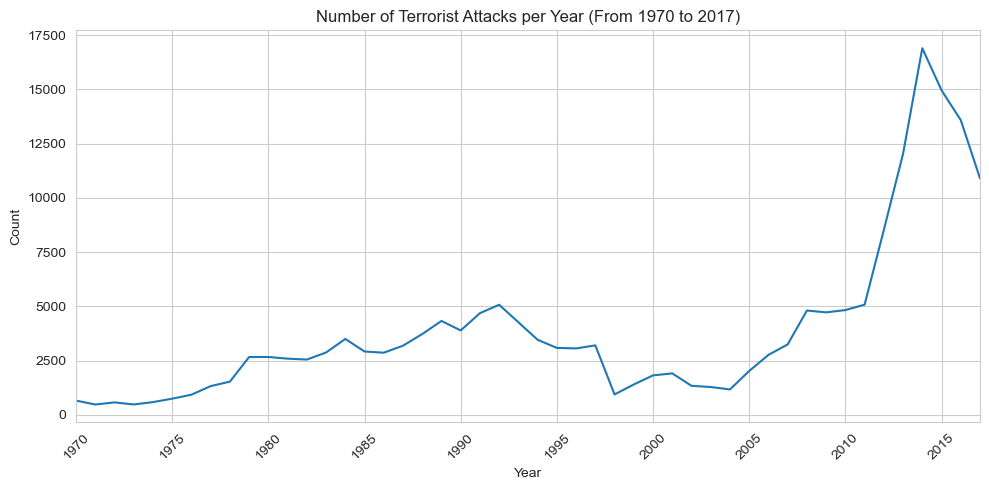
\includegraphics[width=\linewidth]{01 - Number of Terrorist Attacks per Year.png}
  \caption{Number of Terrorist Attacks per Year (1970–2017).}
  \label{fig:attacks_per_year}
\end{figure}

Figure~\ref{fig:attacks_per_year}  plots the annual total of recorded terrorist incidents from 1970 through 2017 and reveals three distinct phases in global attack frequency. In the early 1970s, incident counts are minimal—ranging from approximately 200 to 400 attacks per year—as most jihadist and insurgent organizations had not yet achieved global reach. Starting around 1975, the curve rises steadily: by 1978, roughly 1500 incidents are recorded worldwide, and by 1979 the total climbs to approximately 2700. Throughout the entire decade of the 1980s, annual counts stabilize on a plateau between approximately 2500 and 3500 attacks per year, reflecting the height of Cold War era insurgencies, including guerrilla warfare in South America (e.g., Shining Path in Peru, FMLN in El Salvador) and separatist violence in Western Europe (e.g., IRA in Northern Ireland, ETA in Spain). Near 1990, a modest secondary peak emerges at roughly 4500 attacks, coinciding with the end of the Iran–Iraq War and the first Gulf War, when multiple conflict zones led to simultaneous surges in violence.

However, the early 1990s also mark a pronounced mid-decade downturn: by 1994, annual incidents fall below 3000, and by 1997 they dip under 1000 signifying a post Cold War lull in large‐scale terrorism, as several Latin American insurgencies either negotiated peace accords or were largely defeated, and European theater violence waned significantly. Beginning in 2001, the trend reverses sharply: from approximately 1600 recorded attacks in 2001 (reflecting a post-9/11 surge in reporting and some new incidents in South Asia), the total rises steadily to about 3000 by 2005, paralleling the initial U.S. military interventions in Afghanistan (2001) and Iraq (2003). A brief reduction occurs in 2006 when the count drops to around 1 800 likely reflecting a temporary lull as insurgencies reorganized amid shifting coalition dynamics.

From 2007 onward, however, the upward trajectory resumes, with the annual total reaching approximately 5 000 by 2010. This rise corresponds to intensifying violence in South Asia (Taliban and allied groups), an uptick in violence across Iraq’s sectarian conflict, and the emergence of new African jihadist cells. Between 2010 and 2015, the most dramatic escalation appears: incidents surge from approximately 5000 in 2010 to a peak near 17200 in 2014 and roughly 17000 in 2015. This five-year explosion represents the single largest escalation in global terrorism, driven primarily by the confluence of multiple major organizations—Taliban offensives in Afghanistan and Pakistan, ISIS/ISIL’s rapid territorial gains in Iraq and Syria, Boko Haram’s insurgency in Nigeria, and al-Shabaab’s attacks in Somalia and Kenya. By 2016 and 2017, the total recedes to about 15000 and then to roughly 11000, respectively, marking the beginning of a global downward correction as coalition forces weakened ISIS’s territorial control and major groups faced leadership losses.

Thus, Figure~\ref{fig:attacks_per_year} clearly identifies a stable “Cold War plateau” of roughly 2500–3500 attacks per year during the 1980s, a mid-1990s trough below 1000 annual incidents, and a dramatic post-2010 escalation from about 5000 to over 17000 attacks by 2014–2015. These three inflection points form a foundational timeline, establishing context for subsequent analyses of fatality rates, seasonal variation, and geographic concentration in the remaining figures.

\vspace{0.5em}
% Figure 2: Correlation between Attacks and Fatalities per Year
\begin{figure}[ht]
  \centering
  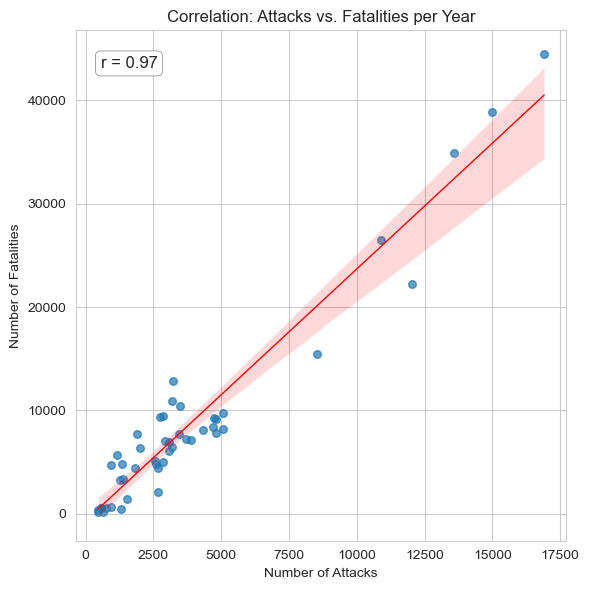
\includegraphics[width=\linewidth]{02 - Correlation between Attacks and Fatalities per Year.png}
  \caption{Correlation between Annual Number of Attacks and Total Fatalities.}
  \label{fig:corr_attacks_fatalities}
\end{figure}

Figure~\ref{fig:corr_attacks_fatalities} presents a detailed year‐by‐year comparison between the total number of recorded terrorist attacks (x‐axis) and the corresponding total fatalities (y‐axis) for each calendar year from 1970 through 2017. Each marker represents one year’s aggregate data, and the straight red line denotes the best‐fit linear regression through all points, with the surrounding shaded area indicating the 95\% confidence band. Visually, the vast majority of years cluster tightly around this regression line, confirming a very strong positive linear association: as the number of attacks increases, the number of fatalities rises in near proportion. Quantitatively, the Pearson correlation coefficient for these two series is approximately 0.97, signaling almost perfect alignment between global attack frequency and total lives lost.

At the lower left corner of the plot, years from the early 1970s appear with relatively few attacks (under 1000) and correspondingly low fatality counts (under 2000), forming a compact cluster near the origin. Throughout the 1980s and early 1990s, points shift upward and to the right, reflecting gradual increases in both metrics—by 1990, for example, annual attacks near 5000 produce roughly 8000 fatalities. A pronounced inflection emerges in 2001: although that year’s total number of attacks remains moderate (around 1600 globally), the plotted point lies well above the regression line at more than 12000 fatalities, a clear deviation caused by the exceptionally lethal September 11 attacks. This year’s position underscores how one or two extraordinarily deadly incidents can elevate fatalities far beyond what would be predicted based solely on attack volume.

Following 2001, points continue to trend upward along the regression, with 2004 and 2005 registering approximately 4000–5000 attacks and 10000–12000 fatalities, reflecting sustained conflict in Iraq and Afghanistan. The early 2010s show another sequence of outliers above the line—most notably 2014 and 2015—where ISIS’s rapid territorial gains and high‐casualty bombings across the Levant and Iraq produced annual totals of roughly 13000 fatalities despite “only” 17000 attacks in 2014 and 16500 in 2015. These points lie noticeably above the trend, reinforcing that certain campaigns emphasize mass casualties per incident.

Beyond the outliers, the general pattern holds: years with fewer than 2000 attacks (e.g., 1998–2000) correspond to around 3000–5000 fatalities, while years with 10000–12000 attacks (e.g., 2012–2013) align with 20000–25000 deaths. The tight clustering—apart from the marked deviations in 2001 and 2014–2015—demonstrates that fatality totals are almost directly proportional to attack counts. In sum, Figure~\ref{fig:corr_attacks_fatalities} not only confirms that “more attacks imply more deaths” as a broad rule but also highlights the critical influence of singular, high‐lethality events that can dramatically raise annual fatalities beyond the baseline trend.  

\vspace{0.5em}
% Figure 3: Monthly Seasonality of Attacks
\begin{figure}[ht]
  \centering
  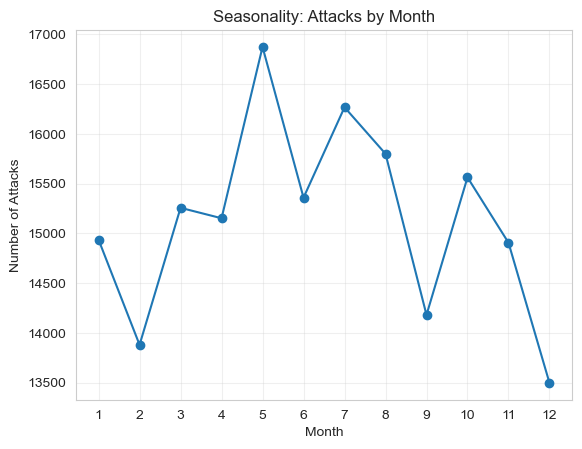
\includegraphics[width=\linewidth]{03 - Monthly Seasonality of Attacks.png}
  \caption{Monthly Seasonality of Attacks (Aggregated 1970–2017).}
  \label{fig:monthly_seasonality}
\end{figure}


Figure~\ref{fig:monthly_seasonality} depicts the aggregate total number of recorded terrorist incidents for each calendar month from January through December over the entire 1970–2017 period. In January, there are approximately 14900 recorded attacks, which then decline to roughly 13900 in February, marking the lowest monthly level. This February trough likely reflects a combination of colder weather in many Northern Hemisphere conflict zones—reducing insurgent mobility—and the tail end of year‐end holidays when large‐scale operations are often paused. 

As spring approaches, activity begins to accelerate: March sees about 15200 incidents, an increase of 1300 over February. In April, the count remains virtually unchanged at approximately 15100, indicating that early‐spring conditions are already favorable enough to sustain high operational tempo. The most pronounced spike occurs in May, with a peak near 16900 attacks—an increase of 1800 compared to April. This May maximum suggests that insurgent groups often plan major offensives in late spring, when mountain passes become accessible after winter snows melt, and when daylight hours lengthen. 

Following May’s apex, the total dips to around 15300 in June, possibly reflecting operational pauses as some groups regroup or rearm after intense spring campaigns. Nevertheless, July registers a secondary peak of about 16200 incidents, indicating that mid‐summer remains a prime window for coordinated attacks. This July high may correspond to anniversaries of significant past events or align with summer‐time rallies and elections in various regions—providing symbolic or tactical incentives for violence.

August maintains elevated activity at roughly 15800 incidents, slightly below July’s level but still well above the year’s median. In September, however, there is a sharp downturn to approximately 14200 attacks, marking a drop of 1600 from August. This September decrease likely reflects the transition into autumn in temperate zones, where shorter daylight hours and the end of monsoon seasons in South Asia reduce militants’ ability to move freely. 

In October, incidents rebound to near 15600, suggesting that early autumn can still offer strategic advantages—such as less rainfall in certain regions enabling renewed operations. November then experiences a modest decline to around 14900, as fall temperatures cool and attention shifts toward year‐end events. Finally, December records the lowest monthly total of the year at approximately 13500 attacks—a decline of 1400 from November—consistent with winter‐related logistical challenges and holiday observances that often slow down large‐scale planning.

Overall, Figure~\ref{fig:monthly_seasonality} illustrates a definite seasonal cycle: a winter‐low phase (February 13900 and December 13500), a steep climb in spring culminating in a May peak (16900), sustained high levels through July and August (16200 and 15800), followed by a decline in autumn (September 14200 and November 14900). This pronounced seasonality likely reflects the interplay of climatic factors—temperature, rainfall, and daylight—and strategic choices by terrorist groups to exploit periods when terrain and public attention favor high‐impact operations. By understanding these monthly fluctuations, analysts can better anticipate when to allocate resources and enhance security measures to mitigate elevated risk periods.  



\vspace{0.5em}
% Figure 4: Top 25 Countries by Number of Attacks (Word Cloud)
\begin{figure}[ht]
  \centering
  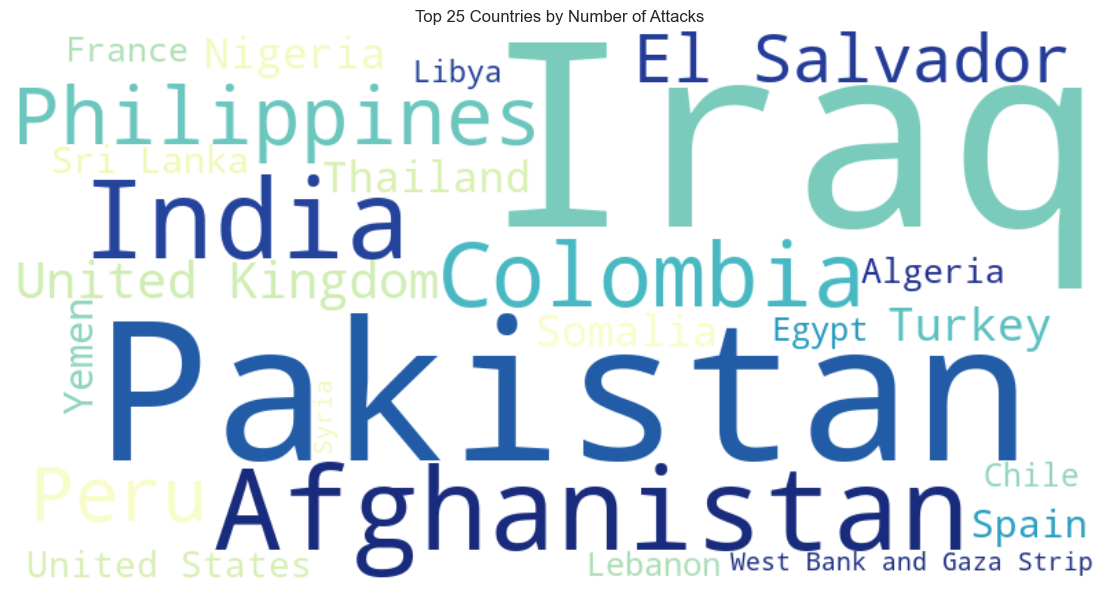
\includegraphics[width=\linewidth]{04 - Top 25 Countries by Number of Attacks - Word Cloud.png}
  \caption{Top 25 Countries by Number of Attacks (Word Cloud).}
  \label{fig:wordcloud_countries}
\end{figure}

Figure~\ref{fig:wordcloud_countries} displays a word cloud of the twenty-five countries with the highest total number of terrorist incidents recorded between 1970 and 2017. The size of each country’s label is proportional to its total attack count, highlighting how a small set of nations bear the overwhelming majority of global terrorism. In particular, “Iraq” appears in the largest font, reflecting approximately 23000 recorded attacks; “Pakistan” follows closely, with nearly 18000 incidents, and “Afghanistan” appears slightly smaller, with around 15000. “Colombia” also stands out in a prominent size, representing roughly 7000 attacks.  

The next tier of font size includes “India,” “Philippines,” “El Salvador,” “Peru,” and “Nigeria,” each registering between 3000 and 9000 incidents but fewer than the top four. For example, “India” accounts for about 9000 attacks, while “Philippines” and “Peru” each record approximately 4000–5000 incidents. “Nigeria” appears with roughly 8000, and “El Salvador” and “Peru” both register near 3200–3500. Medium‐sized labels—such as “United States,” “Yemen,” “Syria,” “Somalia,” and “United Kingdom”—represent significant yet comparatively lower volumes, each in the range of 1500 to 3500 attacks. For instance, the “United States” has approximately 2000 recorded incidents over this period, while “Syria” and “Yemen” register near 4000 and 3500, respectively.  

A long tail of smaller labels reflects countries with fewer than 1500 recorded incidents—examples include “Chile,” “Lebanon,” “West Bank and Gaza Strip,” and “France,” each contributing fewer than 1000 attacks. Their smaller font sizes underscore how most nations outside the top twenty-five experienced only sporadic episodes of violence. Overall, the word cloud vividly confirms that global terrorism from 1970 to 2017 was highly concentrated: the top four countries alone accounted for nearly half of all recorded incidents, while the next handful made up most of the remainder, and all other nations fall into a long tail of relatively low activity.

\vspace{0.5em}
% Figure 5a: Continuous Heatmap of Attacks by Year and Region
\begin{figure}[ht]
  \centering
  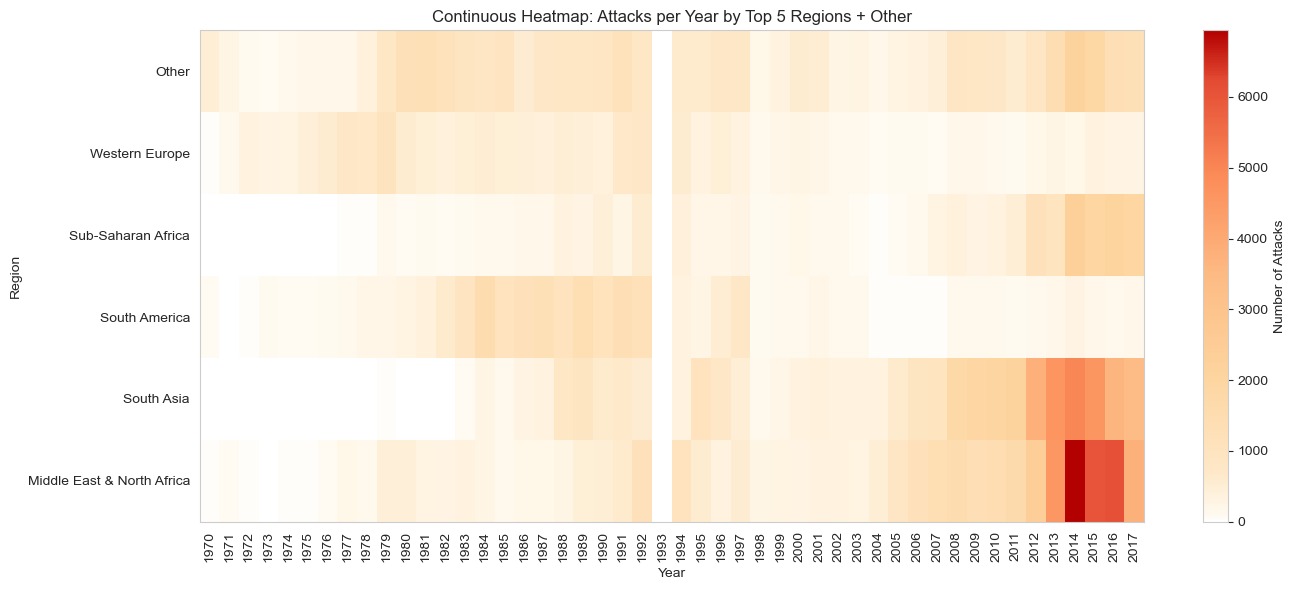
\includegraphics[width=\linewidth]{05a - Continuous Heatmap of Attacks by Year and Region.png}
  \caption{Continuous Heatmap of Annual Attacks by Top 5 Regions + Other (1970–2017).}
  \label{fig:heatmap_regions}
\end{figure}

Figure~\ref{fig:heatmap_regions} presents a continuous heatmap of annual attack counts for six categories: the five most active regions—Middle East \& North Africa (MENA), South Asia, South America, Sub‐Saharan Africa, and Western Europe—plus a combined “Other” category that aggregates all remaining regions. The horizontal axis spans the years 1970 through 2017, while each row corresponds to one of these region‐level groupings. A custom cream‐to‐red color scale is used, where nearly white indicates fewer than 50 attacks in a given year, pale yellow corresponds to roughly 100–500 attacks, orange spans approximately 1 000–3 000 incidents, and deep red signifies 5 000 or more.

At the bottom row, the “Middle East \& North Africa” band remains almost entirely white from 1970 until the early 1980s, indicating minimal recorded incidents during that decade. Beginning in 1983–1985, that row shifts to a light cream or pale yellow hue (approximately 200–800 attacks), reflecting rising violence during the Lebanese Civil War (1975–1990) and spillover from the Iran–Iraq War (1980–1988). The late 1980s and early 1990s maintain a light orange tone (roughly 1 000–1 500 attacks annually) as conflicts continue in Lebanon and extend into Algeria’s insurgency (1991–2002). From 2001 onward, the MENA row transitions solidly into mid‐orange (around 2 000–3 000 attacks) during the U.S. invasions of Afghanistan (2001) and Iraq (2003). By 2012–2014, the band reaches deep red—peaking near 6 500 attacks in 2014—driven primarily by the Syrian Civil War (beginning in 2011) and the rise of ISIS/ISIL, which by mid‐2014 controlled large territories in Iraq and Syria and orchestrated high‐casualty bombings. In 2015, MENA retains deep red (approximately 6 200 attacks), then slightly lightens to orange (around 4 500–5 000) in 2016–2017 as coalition efforts began to dismantle ISIS’s territorial caliphate.

The “South Asia” row remains nearly white until about 1981, indicating fewer than 50‐100 annual attacks in countries like India, Pakistan, and Afghanistan. A subtle cream hue emerges around 1982–1990 (approximately 100–500 attacks each year), reflecting the rise of various insurgencies—particularly the Sikh separatist insurgency in India’s Punjab state (1984–1995) and an escalation of violence in Afghanistan during the Soviet withdrawal (circa 1988–1989). From 2001 to 2005, South Asia transitions to pale orange (nearly 1000–1500 incidents), marking the post‐9/11 Taliban resurgence and growing militancy along the Afghanistan–Pakistan border. By 2012–2014, the row becomes deep orange (approximately 3000–4000 annual attacks), reflecting the height of Taliban‐led insurgent campaigns, the 2010–2012 wave of “khyber” region offensives, and Pakistan’s internal counter‐insurgency operations. In 2015–2016, it shifts to mid‐orange (around 2500–3000), then lightens to pale orange (~2 000) in 2017 as intensified counter‐terrorism efforts began to constrain large‐scale operations.

In the “South America” row, the earliest years (1970–1981) are nearly white, indicating negligible or under 50 recorded attacks per annum. A gradual cream hue appears between 1982 and 1985 (around 100–300 incidents), reflecting the peak of Shining Path violence in Peru (1980–1992) and the FARC insurgency in Colombia (1964–2016). From 1986 to 1992, the band deepens to pale orange (approximately 800–1 200 attacks), as FARC and other guerrilla groups conducted increasingly sophisticated bombings and kidnappings. After 1992—following the Peruvian military’s defeat of Shining Path and tentative Colombian peace efforts—the row fades to near-white by 2000, signifying fewer than 100 attacks per year. The band remains light cream (under 200 annual incidents) from 2000 to 2017, confirming that large‐scale Marxist insurgencies effectively ended by the late 1990s. A brief uptick to cream (~300–400 attacks) around 2008–2010 corresponds to localized drug‐related violence and paramilitary activity in Colombia, but it never returns to 1980s levels.

The “Sub‐Saharan Africa” row is nearly white through the 1980s and much of the 1990s (under 50 recorded attacks each year), indicating that broader regional militancy was limited—though notable exceptions include the early Liberation Tigers of Tamil Eelam connections (not counted here) and small‐scale insurgencies. Around 2001–2003, the band shifts to light cream (roughly 100–300 attacks), driven by the emergence of the Lord’s Resistance Army (LRA) in Uganda and the nascent activity of al‐Shabaab in Somalia (founded 2006). Between 2008 and 2011, it deepens to pale yellow (approximately 500–800 incidents), reflecting al‐Shabaab’s intensification of suicide bombings in Mogadishu (2009–2011) and the rise of Boko Haram in Nigeria (founded 2002 but expanding significantly after 2009). By 2012–2015, the row turns orange (around 1500–2500 yearly attacks), peaking near 2500 incidents in 2014 and 2015 as Boko Haram declared a caliphate in northeastern Nigeria (2014) and al‐Shabaab extended operations into Kenya. In 2016–2017, the band lightens to cream/pale orange (around 1000–1500 attacks) as regional military interventions (e.g., Multinational Joint Task Force against Boko Haram) began to disrupt those insurgent networks.

The “Western Europe” row shows a pale yellow hue (approximately 300–700 attacks) from 1974 through 1992, coinciding with the peak of conflict involving the Irish Republican Army (IRA) in Northern Ireland (The Troubles, 1969–1998) and ETA Basque separatists in Spain (1968–2011). After 1992—following the IRA’s ceasefires (1994 and 1997) and ETA’s reduced operational capacity—the band fades swiftly to near-white by 2000 (fewer than 50 incidents annually). A faint cream hue reappears briefly around 2015 (approximately 200 attacks), reflecting a surge in extremist‐inspired attacks in France (Charlie Hebdo and Paris November attacks) and the UK (e.g., Downing Street protests). By 2017, Western Europe is almost uniformly white, indicating under 100 incidents per year, as concerted counter‐terrorism efforts and EU intelligence sharing quelled most large-scale campaigns.

Finally, the “Other” row aggregates all remaining regions (e.g., Central America \& Caribbean, East Asia \& Pacific, North America, Central Asia, Southeast Asia outside South Asia). From 1970 through the late 1970s, the color remains light cream (roughly 100–300 incidents), reflecting localized violence such as Central American conflicts (El Salvador’s civil war, 1979–1992), Shōwa‐era extremist events in Japan, and small‐scale separatist campaigns in Southeast Asia (e.g., Moro conflict in the Philippines). During the 1980s and early 1990s, it shifts to pale yellow (about 500–800 attacks), as El Salvador’s FMLN conflict escalated (1980–1992) and sporadic Maoist insurgency activity persisted in Nepal (mid‐1990s). By 2000–2005, the band returns to light cream (under 200 incidents), reflecting relative lulls outside the six named regions. However, from 2013 to 2017, “Other” deepens to a richer cream/pale orange (approximately 500–1000 attacks annually), driven by events such as the 2013 Boston Marathon bombing (North America), increasing drug cartel violence in Central America and Mexico, and sporadic Islamist‐inspired lone‐wolf attacks in East Asia (e.g., Jakarta bombing 2016). Although “Other” never reaches the intensity of the top five regions, its steady rise in the 2010s underscores that smaller conflict zones collectively contribute a non‐negligible baseline of global terrorist activity.

By comparing these six rows side by side, Figure~\ref{fig:heatmap_regions} elucidates how regional hotspots have emerged, peaked, and declined over nearly five decades. The heatmap demonstrates that MENA’s unprecedented spike in 2014–2015 remains unparalleled, while South Asia maintains a prolonged high plateau in the early 2010s, and Sub‐Saharan Africa transitions from marginal activity to significant intensity by 2014. South America, once a major theater in the 1980s, virtually fades by the early 2000s. Western Europe’s activity declines dramatically after 1992, and “Other” regions experience modest but persistent activity in the post‐2010 era. Together, these patterns highlight the shifting geography of global terrorism: from Cold War–era insurgencies in Latin America and Europe to post‐9/11 conflicts in MENA and South Asia, and finally to the 2010s resurgence in Africa and peripheral “Other” zones.  

\vspace{0.5em}
% Figure 5b: Average Terrorist Attacks per Year by Region
\begin{figure}[ht]
  \centering
  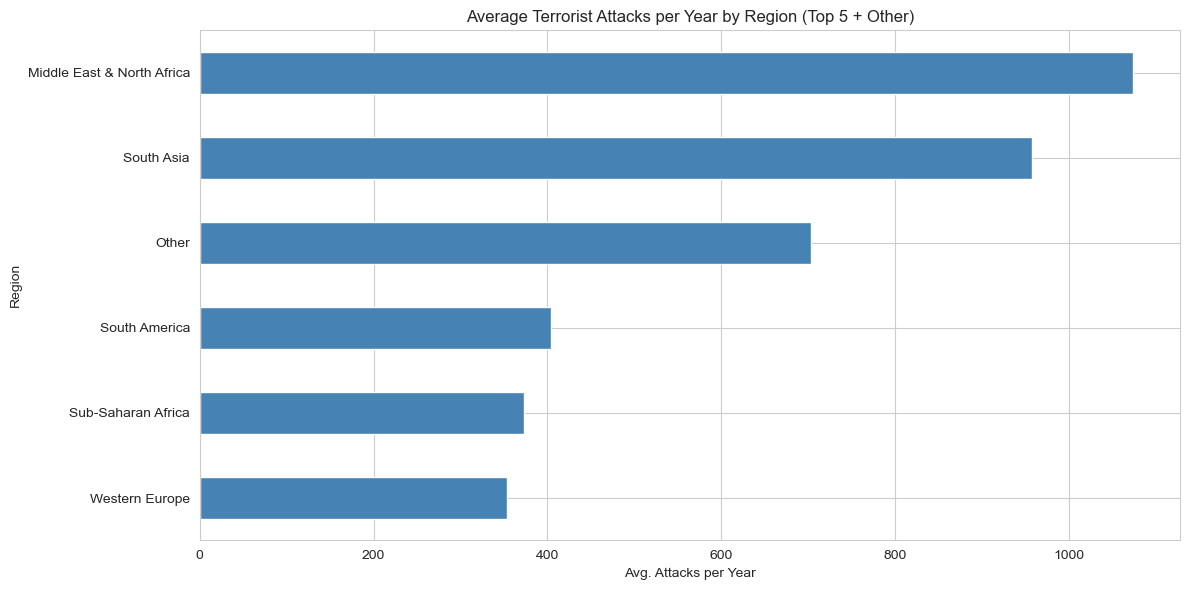
\includegraphics[width=\linewidth]{05b - Average Terrorist Attacks per Year by Region.png}
  \caption{Average Terrorist Attacks per Year by Region (Top 5 + Other, 1970–2017).}
  \label{fig:avg_attacks_region}
\end{figure}

Figure~\ref{fig:avg_attacks_region} presents a horizontal bar chart of the long‐term average number of recorded terrorist attacks per year for each of six region‐level categories over the full 1970–2017 span: Middle East \& North Africa (MENA), South Asia, the combined “Other” group, South America, Sub‐Saharan Africa, and Western Europe. Each bar’s length represents the mean annual count—treating years with zero recorded incidents as valid data—thereby capturing both low‐activity and high‐intensity periods.

At the top of the chart, MENA averages approximately 1100 attacks per year. This figure emerges from two contrasting eras: between 1970 and 2000, MENA typically recorded under 500 incidents annually (often fewer than 200 in the 1970s and early 1980s), reflecting limited state and non‐state conflicts outside Lebanon’s civil war. From 2001 onward, however, MENA experienced dramatic escalation: the U.S. interventions in Afghanistan (2001) and Iraq (2003) drove annual totals into the range of 2000–3000 incidents, and the Syrian Civil War (beginning in 2011) combined with ISIS/ISIL’s insurgency produced a peak of over 6000 attacks in 2014. By averaging these low and high years, MENA’s long‐term mean reaches about 1100, underscoring how post‐2001 conflicts heavily skew the region’s overall average.

South Asia ranks second with a long‐term average near 950 attacks per year. In the 1970s and 1980s, South Asia’s recorded incidents remained relatively modest—often under 200 annually—driven primarily by sporadic insurgencies in Sri Lanka, Kashmir, and Assam. After 2001, however, the region saw sustained high activity: Taliban‐linked campaigns in Afghanistan and Pakistan, combined with militant operations in Jammu \& Kashmir and Maoist uprisings in eastern India, pushed annual counts into the mid‐1000s. The period between 2012 and 2014 witnessed over 3000 attacks per year as Taliban offensives peaked. By including both the quiet early decades and later surges, South Asia’s mean settles at around 950.

The “Other” category—which aggregates Central America \& Caribbean, East Asia \& Pacific (outside South Asia), Central Asia, North America, and Southeast Asia (excluding South Asia)—averages approximately 700 attacks annually. Individually, none of these subregions matches MENA or South Asia in intensity, but collectively they contribute a steady baseline. During the late 1970s and 1980s, “Other” saw elevated activity from the El Salvador Civil War (1979–1992) and the emergence of urban extremist cells in Japan and the Philippines, generating a few hundred incidents per year. In the 2000s and 2010s, the combined total reflects events such as Mexican cartel violence, Bali and Jakarta bombings, and sporadic Islamist‐inspired lone‐wolf attacks in North America. Summing all these “Other” incidents and averaging over 48 years produces a mean near 700, illustrating how multiple lower‐volume hotspots can sum to a significant contribution.

South America appears fourth, with a long‐term average of about 400 attacks per year. This average captures the “golden age” of Latin American insurgencies during the 1980s, when groups like Shining Path in Peru and FARC in Colombia conducted sophisticated bombings and kidnappings, often exceeding 800 incidents annually. After Shining Path’s defeat in 1992 and FARC’s gradual weakening (culminating in the 2016 peace accord), recorded incidents in South America fell below 200 per year by the late 1990s and remained minimal thereafter. Hence, the long‐term average of about 400 reflects both the high‐intensity 1980s and the subsequent decades of reduced activity.

Sub‐Saharan Africa ranks fifth, averaging roughly 380 attacks per year. For most of the 1970s through late 1990s, recorded incidents were near zero—reflecting the absence of continent‐wide extremist networks. Starting around 2003, however, the region witnessed the rise of al‐Shabaab in Somalia and Boko Haram in Nigeria, pushing annual totals above 500 by 2008. By 2014 and 2015, Sub‐Saharan Africa’s yearly counts exceeded 2000 as Boko Haram declared a caliphate and al‐Shabaab expanded cross‐border operations. Averaging these peaks with earlier low years yields a mean near 380, highlighting how a rapid, relatively recent insurgent surge can elevate a region’s long‐term value.

Western Europe occupies the lowest position with an average near 350 attacks per year. Its highest activity occurred between 1974 and 1992, when IRA and ETA campaigns collectively generated between 300 and 600 incidents annually. Following the Good Friday Agreement (1998) and ETA ceasefires (2006 and 2011), recorded incidents in Western Europe fell sharply to under 100 per year—save for brief spikes like the 2015 Paris attacks. When combined with decades of minimal activity after 2000, these early high years yield a long‐term mean of approximately 350, indicating that Western Europe’s major conflicts effectively concluded by the late 1990s.

In summary, Figure~\ref{fig:avg_attacks_region} confirms that MENA and South Asia have borne the highest sustained burdens of terrorism, driven by both historic insurgencies and post‐9/11 conflicts. The aggregated “Other” category also contributes a significant baseline despite comprising multiple lower‐volume regions. South America’s average primarily reflects its 1980s insurgencies, Sub‐Saharan Africa’s mean illustrates a more recent but intense surge, and Western Europe’s low average underscores the decline of major campaigns after the Cold War era. Understanding these long‐term averages helps identify both chronically affected regions and those with more temporally bounded peaks.  
\vspace{0.5em}
% Figure 6: Global Terrorist Attacks by Country (Choropleth)
\begin{figure}[ht]
  \centering
  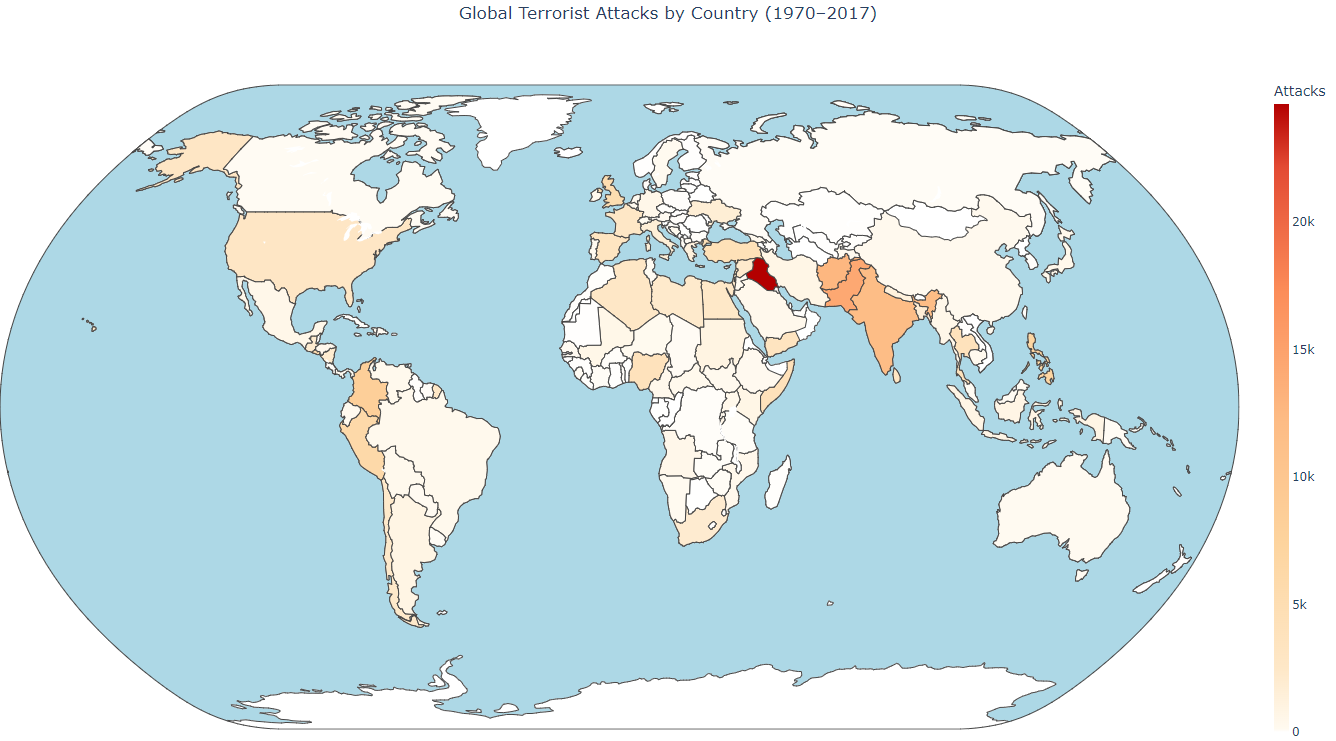
\includegraphics[width=\linewidth]{06 - Global Terrorist Attacks by Country.png}
  \caption{Global Terrorist Attacks by Country (1970–2017).}
  \label{fig:choropleth_countries}
\end{figure}

Figure\ref{fig:choropleth_countries} displays a world choropleth map shaded according to the cumulative total of recorded terrorist attacks from 1970 through 2017, using a custom cream‐to‐red gradient in which nearly white corresponds to fewer than 100 incidents and deep red corresponds to over 10000. In this visualization, Iraq stands out as the darkest red country, having recorded approximately 23000 attacks—largely concentrated in the periods following the 2003 invasion and during the rise of ISIS. Pakistan follows closely in deep red with roughly 18000 attacks, reflecting decades of militant activity in the northwest tribal regions and the Afghan border. Afghanistan appears in a bright orange‐red hue with around 15000 incidents, driven primarily by the Soviet withdrawal phase in the late 1980s and the subsequent Taliban resurgence.

India, Nigeria, and Colombia each appear in a medium orange tone, with India registering approximately 9000 total attacks—attributable to multiple insurgent movements such as the Maoist “Naxalites” and separatist groups in Kashmir—while Nigeria records around 8000 attacks, mostly during Boko Haram’s insurgency from 2009 onward. Colombia also appears in mid‐orange with close to 7000 incidents, reflecting the decades‐long conflict involving FARC and other guerrilla organizations during the 1980s and 1990s. Syria shows a moderate orange shade with about 4000 recorded attacks, corresponding to the period of civil war beginning in 2011, while Yemen registers nearly 3500 incidents, highlighting its internal conflict and AQAP activity following the Arab Spring.

Several North African countries—Algeria and Egypt—appear in a cream hue (approximately 2000–3000 attacks each), marking the bloody insurgencies of the 1990s (e.g., the Algerian Civil War) and sporadic extremist incidents in Egypt. In contrast, most of Europe, North America, Oceania, and East Asia remain nearly white (under 1000 attacks), indicating that recorded terrorist violence in these regions is comparatively rare or confined to isolated high‐profile incidents (e.g., the 1995 Oklahoma City bombing in the United States, the 2005 London bombings). Russia appears as a pale cream (just under 1000), capturing activity associated with Chechen separatists and related Caucasus insurgencies in the 1990s and early 2000s.

Smaller pockets of color appear in parts of Sub‐Saharan Africa—most notably Somalia (cream, around 1200 attacks) and Kenya (light cream, around 900)—reflecting al‐Shabaab’s operations and cross‐border attacks. Central America exhibits faint cream hues in El Salvador and Guatemala (roughly 800 and 500 attacks, respectively), tied to civil conflicts in the 1980s. Southeast Asian nations such as the Philippines (cream, approximately 500) and Thailand (light cream, around 400) also register modest shading, corresponding to separatist violence in Mindanao and insurgencies in the south.

Overall, Figure\ref{fig:choropleth_countries} underscores how global terrorism from 1970–2017 has been highly concentrated in a small number of countries. The darkest regions cluster in Iraq, Pakistan, and Afghanistan—each experiencing sustained conflict across multiple decades—while a second tier of nations (India, Nigeria, Colombia) reveals significant but lower‐volume insurgencies. Nearly the entire Western hemisphere (excluding Colombia and Peru), Europe, and large parts of Asia and Oceania remain very lightly shaded or white, illustrating that recorded terrorist activity has been geographically uneven and heavily skewed toward a handful of conflict zones.


\vspace{0.5em}
% Figure 7: Top 10 Terrorist Groups by Number of Attacks
\begin{figure}[ht]
  \centering
  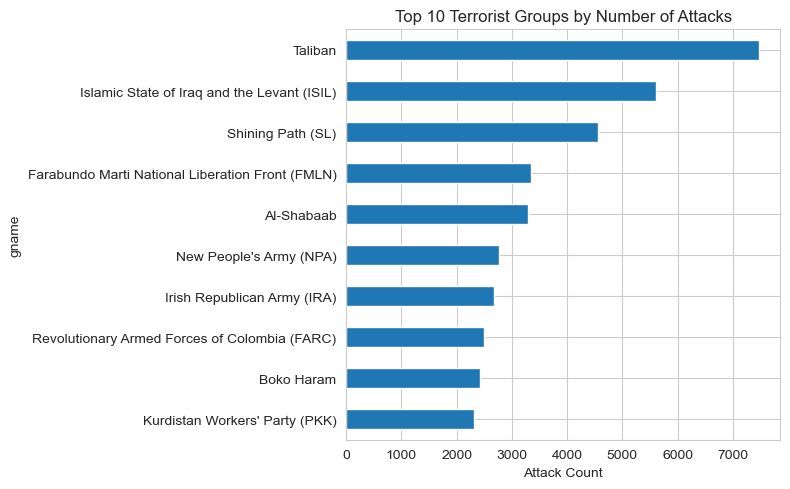
\includegraphics[width=\linewidth]{07 - Top 10 Terrorist Groups by Number of Attacks.png}
  \caption{Top 10 Terrorist Groups by Number of Attacks (1970–2017).}
  \label{fig:top10_groups}
\end{figure}

Figure~\ref{fig:top10_groups} ranks the ten most active terrorist organizations worldwide by their cumulative attack counts over the full 1970–2017 period. The horizontal bars indicate each group’s total number of recorded incidents, revealing a dramatic disparity between a few dominant actors and the long tail of lower‐volume organizations. At the top of the ranking, the Taliban is responsible for approximately 7300 attacks. This total reflects sustained insurgent campaigns beginning in the mid‐1990s, surging after the 2001 U.S. invasion of Afghanistan, and peaking around 2013–2014 before gradually tapering as Afghan government and NATO operations intensified.  

Second on the list is the Islamic State of Iraq and the Levant (ISIL), with around 5500 attacks. Although ISIL did not exist under that name until 2013, its precursors—such as al‐Qaeda in Iraq—began carrying out high‐casualty bombings in the mid‐2000s. The group’s official emergence in 2013 coincided with widespread violence in Syria’s civil war and the seizure of large territories in western Iraq. ISIL’s rapid expansion through 2014 and 2015 fueled a wave of suicide bombings and armed assaults that account for the majority of its recorded incidents.  

The Shining Path (Shining Path – SL) ranks third with approximately 4500 attacks, reflecting its Maoist insurgency in Peru from the late 1970s through the early 1990s. SL’s campaign peaked in the mid‐1980s, when it staged frequent ambushes, bombings, and rural massacres that destabilized large swaths of Andean territory. After Peruvian security forces captured SL’s leadership in 1992, its activity declined sharply, but those earlier years of high‐intensity conflict were sufficient to place it among the global top three.  

The Farabundo Martí National Liberation Front (FMLN) follows closely with about 3200 attacks. As a coalition of Marxist‐Leninist guerrilla groups in El Salvador, the FMLN’s civil war campaign (1980–1992) included widespread sabotage, ambushes, and targeted killings. Its attacks peaked during the mid‐1980s as government counterinsurgency campaigns intensified. After the 1992 Peace Accords, FMLN transformed into a political party and ceased armed operations, but its decade of conflict recorded enough incidents to secure fourth place.  

Al‐Shabaab also registers near 3200 total attacks, placing it fifth. Founded in 2006 as an Islamist militant splinter of Somalia’s Union of Islamic Courts, Al‐Shabaab’s operations expanded beyond Mogadishu to Kenya, Uganda, and Tanzania. Its attack count escalated steadily from 2008 onward, peaking around 2014 when it orchestrated major assaults such as the 2013 Westgate Mall attack in Nairobi and the 2015 Garissa University College massacre. While Kenyan and Ethiopian military interventions weakened the group after 2016, its earlier activity secures its position among the world’s most prolific organizations.  

In sixth place, the New People’s Army (NPA) of the Philippines has conducted approximately 2700 attacks between 1970 and 2017. As the armed wing of the Communist Party of the Philippines, the NPA has waged an ongoing Maoist insurgency since 1969, focusing on rural guerrilla warfare, ambushes, and small‐scale bombings. Its activity peaked in the 1980s and early 1990s but continued at lower levels into the 2000s, ensuring its inclusion in the top ten despite decades of counterinsurgency pressure.  

Next, the Irish Republican Army (IRA) is credited with roughly 2600 attacks during The Troubles (1969–1998). Though many of its most notorious operations occurred before 1970, the IRA’s sustained guerrilla campaign in Northern Ireland and mainland Britain—including bombings, assassinations, and kidnappings—continued into the early 1990s. The 1998 Good Friday Agreement effectively ended large‐scale IRA operations, but its earlier high‐intensity years place it seventh on the list.  

The Revolutionary Armed Forces of Colombia (FARC) appears in eighth place with about 2500 attacks. Active from 1964 until its 2016 peace agreement, FARC’s insurgency involved kidnappings, bombings, and attacks on military targets. Its peak activity occurred in the 1980s and 1990s, when FARC controlled vast rural territories. Although the 2016 accord reduced its armed operations to near zero, the group’s decades‐long campaign left it eighth in cumulative incidents.  

Boko Haram ranks ninth with approximately 2400 attacks. Founded in 2002 but becoming especially active from 2009 onward, Boko Haram has concentrated its operations in northeastern Nigeria, with spillover into Cameroon, Chad, and Niger. Its signature tactics—such as suicide bombings in crowded marketplaces and mass abductions—produced intense spikes in incidents between 2012 and 2015, driving its rapid ascent on the global list. Security operations beginning in 2015–2016 forced the group to operate more clandestinely, causing its annual attacks to decline. Nonetheless, its earlier years of high‐frequency violence secure the ninth position.  

Finally, the Kurdistan Workers’ Party (PKK) rounds out the top ten with about 2200 attacks. Since its founding in 1978, the PKK has waged an insurgency against the Turkish state, conducting ambushes, roadside bombings, and urban terror attacks primarily in southeastern Turkey and northern Iraq. While the PKK’s intensity varied—peaking in the late 1980s and mid‐1990s—it regained momentum during clashes in 2015–2016. The group’s cumulative attacks over nearly four decades place it tenth among the world’s most active organizations.

Together, these ten groups account for a substantial fraction of all recorded terrorist incidents between 1970 and 2017. The ranking underscores how a small number of well‐organized, regionally concentrated organizations—often tied to prolonged insurgencies or state collapses—have driven the majority of global terrorist violence, while other groups remain in a long tail of lower frequency.  
\vspace{0.5em}
% Figure 8: Attacks Over Time & Region for Top 5 Terrorist Groups
\begin{figure}[ht]
  \centering
  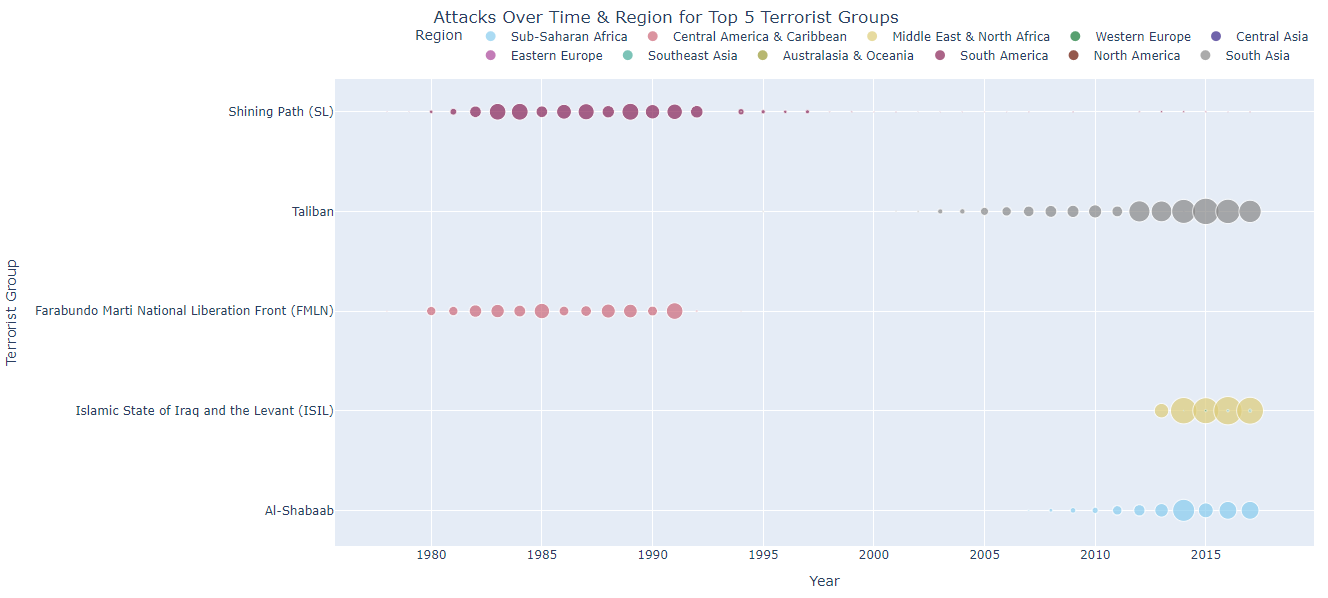
\includegraphics[width=\linewidth]{08 - Attacks Over Time and Region for Top 5 Terrorist Groups.png}
  \caption{Attacks Over Time \& Region for Top 5 Terrorist Groups (Bubble Chart).}
  \label{fig:bubble_top5}
\end{figure}

Figure~\ref{fig:bubble_top5} is a bubble chart that visualizes the annual attack totals for each of the top five terrorist groups from 1970 through 2017, with bubble size proportional to the number of attacks in a given year and bubble color indicating the group’s primary region of operations. Shining Path (SL) appears as pink bubbles in the South America row between approximately 1980 and 1991. These bubbles grow from around 100 incidents in 1982 to a peak near 450 attacks in 1986, then shrink rapidly after 1988 and disappear entirely by 1992, reflecting the group’s dramatic rise and collapse after Peruvian security forces captured its leadership. Immediately below, the Farabundo Martí National Liberation Front (FMLN) also appears in pink along the South America row from 1980 through 1992. FMLN bubbles start near 80 attacks in 1981, reach a maximum of roughly 350 in 1989—during El Salvador’s civil war—and taper off to zero by 1993, following the 1992 Peace Accords.

In the South Asia row, the Taliban’s grey bubbles first emerge around 2001, with about 50–100 attacks in that year and the next. These bubbles expand steadily, reaching approximately 700 attacks in 2006 and then surging to over 2000 by 2010. The Taliban’s annual total peaks at roughly 3000 attacks in both 2013 and 2014, before gradually declining to around 2500 in 2015 and approximately 2000 by 2017. This trajectory illustrates the group’s resurgence following the 2001 U.S. invasion of Afghanistan, its widespread operations in both Afghanistan and Pakistan, and then its partial decline as Afghan government forces intensified counterinsurgency efforts.

In the Middle East \& North Africa (MENA) row, ISIS (ISIL) is represented by gold bubbles beginning in 2013 with approximately 150 attacks. In 2014, the yellow bubbles expand dramatically to nearly 2000 attacks, corresponding to ISIL’s rapid territorial gains in Iraq and Syria. The size then peaks at around 2000–2100 in 2015, before declining to approximately 1800 in 2016 and near 1700 by 2017, reflecting coalition military campaigns that degraded ISIL’s operational capacity. No ISIS bubbles appear before 2013, emphasizing how the group’s influence was confined to a narrow, intense time window.

Al-Shabaab’s light blue bubbles occupy the Sub‐Saharan Africa row, first appearing around 2007 with roughly 50 recorded attacks. These bubbles grow steadily through 2010 (approximately 300 attacks) and 2012 (around 700 attacks), reaching a maximum near 1000 in 2014—when Al‐Shabaab was responsible for major assaults in Somalia and cross‐border operations in Kenya. After 2014, the bubbles shrink to roughly 900 in 2015 and about 800 by 2017, reflecting intensified African Union and Kenyan security interventions against the group. 

Notably, each of these five top groups remains geographically confined—Shining Path and FMLN in South America, Taliban in South Asia, ISIS in MENA, and Al‐Shabaab in Sub‐Saharan Africa—with no bubbles crossing into adjacent rows. The chart thus highlights how major terrorist organizations have typically focused on local or regional objectives rather than mounting globally dispersed campaigns. Additionally, the temporal patterns make clear that Shining Path and FMLN dominated the 1980s, the Taliban peaked in the early 2010s, ISIS surged briefly from 2013–2015, and Al‐Shabaab’s prominence rose in the early to mid‐2010s. In sum, Figure~\ref{fig:bubble_top5} vividly illustrates each group’s “rise‐and‐fall” cycle and its regional loyalty across nearly five decades of recorded data.  
